\documentclass[twoside,a4paper,12pt]{book}
\usepackage[twoside,a4paper,top=2.5cm, left=2cm, width=17cm, height=22.5cm]{geometry}
\usepackage[utf8]{inputenc}
\usepackage{graphicx}
\usepackage{float}
\usepackage{appendix}
\usepackage{fancyhdr}
% package for providing the size of columns on tables
\usepackage{array}
\usepackage{xcolor}
\usepackage{color}
% Package for avoiding the issue with the option hidelinks of the package hyperref
\usepackage[colorlinks=true,
            linkcolor=black,
            urlcolor=blue,
            citecolor=black,
            hyperfootnotes=true]{hyperref}
\usepackage{caption}
\usepackage{eurosym}
\usepackage{multirow}
% Package for providing highlights on code
\usepackage{listings}
\usepackage[nohyperlinks,smaller,withpage]{acronym} 
\usepackage{enumitem}
\usepackage[acronym]{glossaries}
\usepackage{mathtools}
% Package for version history
\usepackage{vhistory}
\DeclarePairedDelimiter{\ceil}{\lceil}{\rceil}

\newcommand{\ada}[1]{\lstinline[style=ada,
keywordstyle=\mdseries,breaklines,backgroundcolor=\color{white}]&#1&}
\newcommand{\asm}[1]{\lstinline[style=sparc,
keywordstyle=\mdseries,breaklines,backgroundcolor=\color{white}]$#1$}
\newcommand{\prog}[1]{\asm{#1}}

\definecolor{dkgreen}{rgb}{0,0.6,0}
\definecolor{gray}{rgb}{0.8,0.8,0.8}
\definecolor{mauve}{rgb}{0.58,0,0.82}
\definecolor{purple2}{RGB}{153,0,153} % there's actually no standard purple
\definecolor{green2}{RGB}{0,153,0} % a darker green

% Define column type for vertical and horizontal alignment
\newcolumntype{M}[1]{>{\centering\arraybackslash}m{#1}}

% json style
\lstset{
    string=[s]{"}{"},
    stringstyle=\color{blue},
    comment=[l]{:},
    commentstyle=\color{black},
}

\lstdefinestyle{xml}{
       language=xml,
        basicstyle=\ttfamily,
        aboveskip= \bigskipamount,
        belowskip= \bigskipamount,
        abovecaptionskip= \medskipamount,
        belowcaptionskip=\bigskipamount,
        xleftmargin=\parindent,
        columns=flexible,
        numbers=left,
        breaklines=true,
        showstringspaces=false
}


\lstdefinestyle{bash}{
       language=bash,
        basicstyle=\ttfamily,
        aboveskip= \bigskipamount,
        belowskip= \bigskipamount,
        abovecaptionskip= \medskipamount,
        belowcaptionskip=\bigskipamount,
        xleftmargin=\parindent,
        columns=flexible,
        showstringspaces=false,
        breaklines=true,
        showstringspaces=false
}

\lstdefinestyle{python}{%
  language=Python,                   % the language
  basicstyle=\ttfamily,   % size of the fonts for the code
  % Color settings to match IDLE style
  keywordstyle=\color{orange},       % core keywords
  keywordstyle={[2]\color{purple2}}, % built-ins
  stringstyle=\color{green2},
  commentstyle=\color{red},
  upquote=true,                      % requires textcomp,
  numbers=left,
  breaklines=true,
  showstringspaces=false
}


\makeglossaries


\begin{document}

\newacronym{eboa}{E-BOA}{Engine for Business Operation Analysis}

\newacronym{rdbms}{RDBMS}{Relational Database Management System}

\newacronym{uuid}{UUID}{Universally unique identifier}

\newacronym{pid}{PID}{Process identifier}


\newglossaryentry{leon2}{name={LEON2},
    description={Es un core de microprocesador de 32-bits basado en la
    arquitectura RISC y en el conjunto de instrucciones SPARC V8. Originalmente
    diseñada por la \gls{esa}, y
    posteriormente por Gaisler Research
    }}


\pagestyle{empty}
% -*-front.tex-*-
%
% Cover page for the GSDM documentation
%
% Written by DEIMOS Space S.L. (dibb)
%
% module gsdm

\begin{titlepage}
	
    
\includegraphics[scale=0.20]{../fig/deimos_logo.jpg}
    
    \vspace{2.0cm}
    
    	\begin{center}
    
    \vspace{2cm}
    
    \LARGE{\textbf{GSDM: Ground Segment Data Management}} \\    
    \LARGE{Dynamic data modelling for ground segment data management facilities}
    
    	\end{center}    
    
    \vspace{7.0cm}

    \vspace{0.5cm}

    \Large{\textbf{GSDM release:} 0.1.0}

    \Large{\textbf{Document release:} 1.0}

    \vspace{1cm}
    
    \large{Date: \today}
    
\end{titlepage}

\cleardoublepage

\setcounter{page}{1}
\pagenumbering{roman}

\frontmatter % Introduction, indexes ...

% Introduction
\begin{versionhistory}
  \vhEntry{1.0}{04.09.2018}{DIBB}{Document created}
\end{versionhistory}


\tableofcontents
\listoffigures
\listoftables

\mainmatter
\pagestyle{fancy}
\fancyhead{}
\fancyhead[RE]{\slshape \rightmark} 
\fancyhead[LO]{\slshape \leftmark}  
\fancyfoot{}
\fancyfoot[C]{\lowercase{\thepage}}
\setlength{\headheight}{15pt}

% Introduction
\chapter{Introduction}\label{c:intro}

\acrshort{eboa} is the component aimed to serve as data storage management for business operation analysis. The component aims to allow a dynamic data structure for reducing the effort of developing data models and managing the complex relations between data received.

All the information received is stored into the database using the following high-level entities:

\begin{itemize}

\item Explicit reference: identifier referring to an entity business-related
\item Event: period of time associated to a gauge of a certain aspect business-related
\item Annotation: particular aspect associated to an explicit reference
\item Input: block of information received from the external interface to process. After the processing, the interesting information is extracted and stored inside the system.
\item Alert: notification to users regarding anomalies identified by the system related to previous entities.
\item Report: container of analysis.

\end{itemize}


% Purpose and scope
\chapter{Purpose and scope}

This component manages the storage of the data received following the next requirements:

\begin{itemize} 

\item Traceability of all the data to the source of information (even information created within the infrastructure)

\item No pre-configuration needed for inserting data

\item Include modern datatypes for storing the data

\item Flexible structure for linking information to events and annotations

\item Flexible structure for linking events between them

\item Flexible structure for linking explicit references between them

\item Continuous developtment/Continuous integration approach

\item Include geo-query functionalities

\item Parallel insertion of data using the \acrshort{rdbms} parallelism mechanisms

\item Quick access to the information by which it can be managed dynamically depending on the needs of the users

\end{itemize}

The scope of this component targets systems/tools with the need of storing time-tagged information. The data model used allows quick access to the information in a structured way.


% Data model
\chapter{Data model}

The \acrshort{gsdm} implements the data model shown in the figure \ref{fg:gsdmdb}.

\begin{figure}[ht]
  \begin{center}
	\centering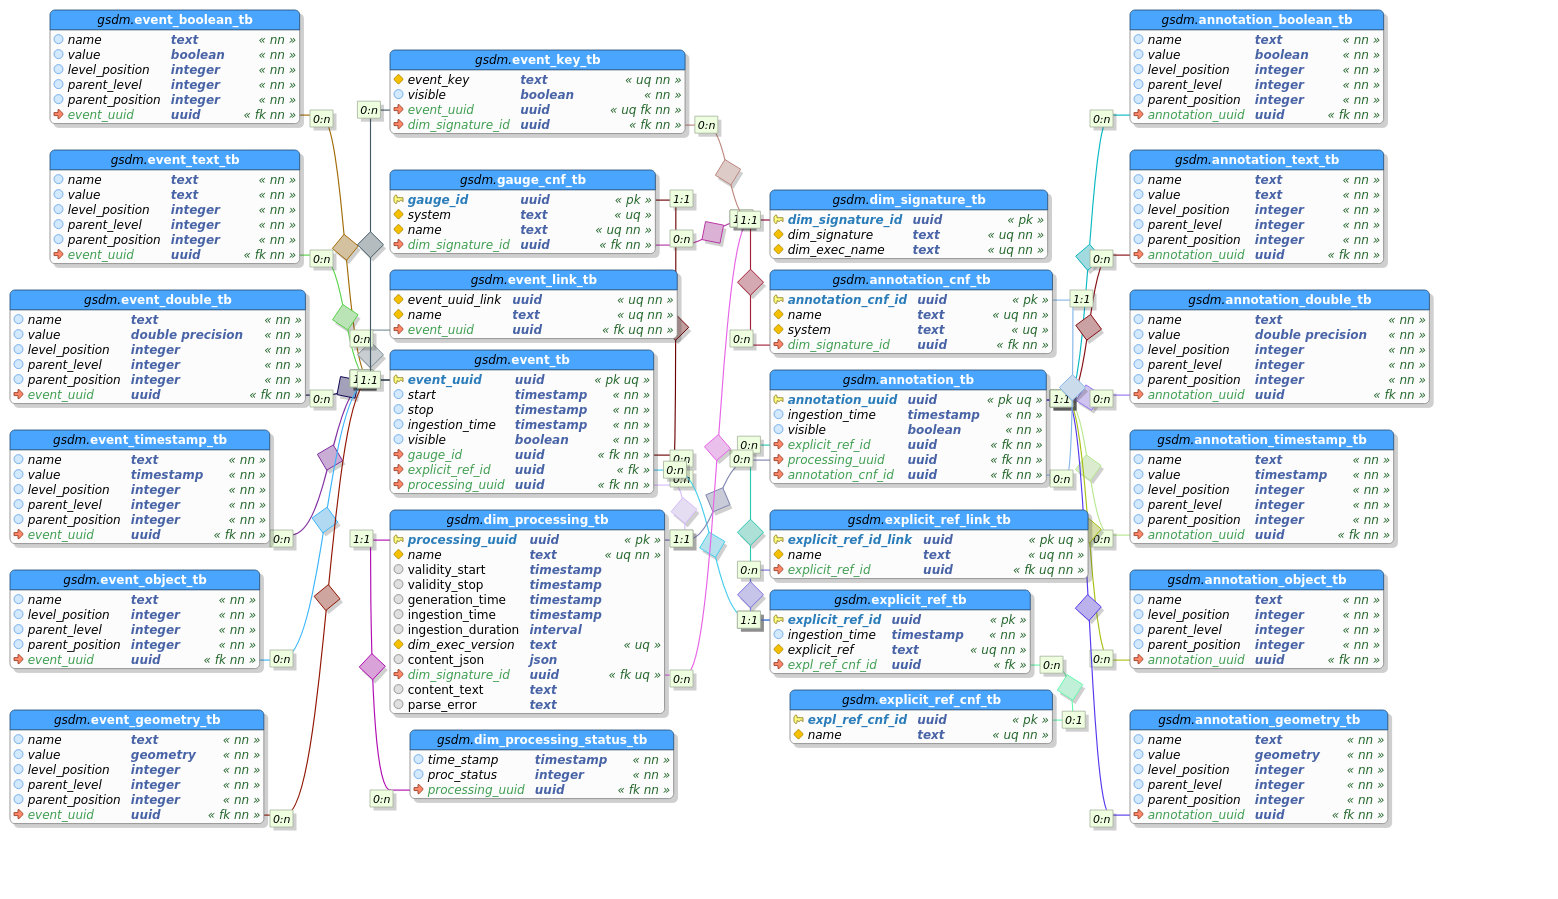
\includegraphics[width=150mm]{../fig/gsdmdb.png}
	\caption{Data model of the \acrshort{gsdm}}
	\label{fg:gsdmdb}
  \end{center}
\end{figure}

As said in chapter \ref{c:intro}, there are 4 main entities in the data model: explicit references (explicit\_ref\_tb), events (event\_tb), annotations (annotation\_tb) and inputs (dim\_processing\_tb).

The entities event and annotation may have an associated dynamic structure of values. These values indicate properties/information of the related entities interesting for the data model. These values are structured in the database following the schema of the figure \ref{fg:values_structure}.

\begin{figure}[ht]
  \begin{center}
	\centering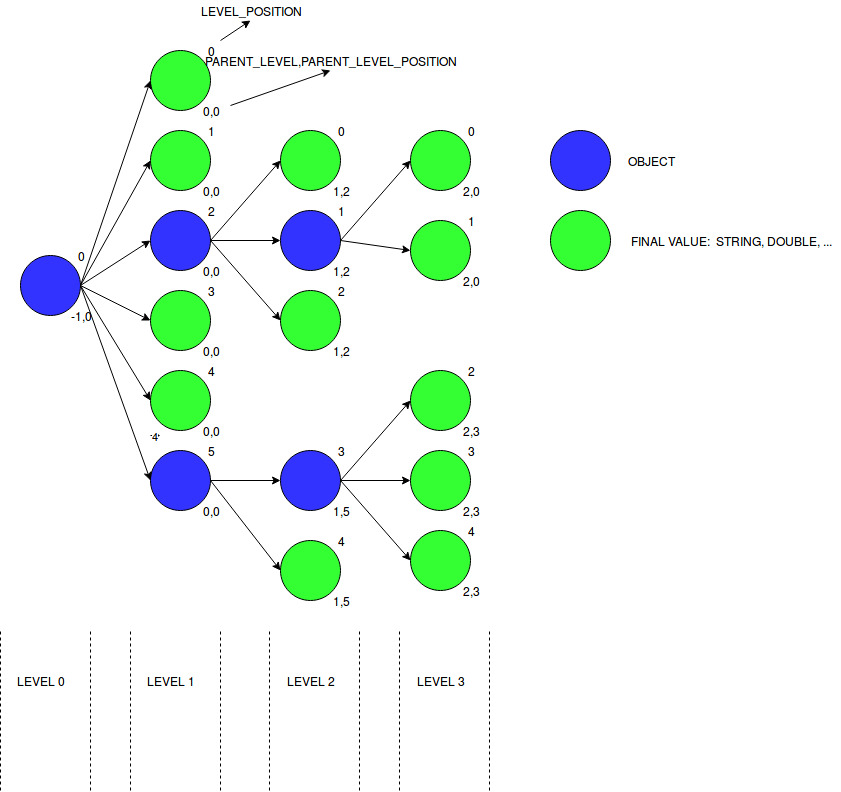
\includegraphics[width=150mm]{../fig/values_structure.jpg}
	\caption{Structure of the values associated to events and annotations}
	\label{fg:values_structure}
  \end{center}
\end{figure}

The values associated to an entity may have one of the following types:

\begin{itemize}

\item Boolean
\item Text
\item Double
\item Timestamp
\item Geometry
\item Object

\end{itemize}

The type object allows every entity to have an associated structure of values (containing other objects). This structure is defined like a tree, every node of the tree may have any of the types described in the previous list. If the node has the type object, the branch has to continue till the final node has a type different than the type object.
The way the tree is structured is as follows:

\begin{enumerate}

\item Every node has a level position
\item Every node has a reference to its parent represented by the parent level and parent level position values
\item Every parent node has the type object
\item Every final node of a branch has a type different than the type object

\end{enumerate}

To better understand how the structure of values is managed by the \acrshort{gsdm}, here it is an example:

Input:
\begin{lstlisting}[breaklines=true, style=xml, caption={XML input example for showing the values structure management.}]
<gsd>
  <insert>
    <dim_signature
        name="test_dim_signature1"
        version="1.0"
        exec="test_exec1"/>
    <source
        name="test_simple_update.xml" 
        generation_time="2018-06-06T13:33:29"
        validity_start="2018-06-05T02:07:03"
        validity_stop="2018-06-05T02:07:36"/>
    <data>
      <event start="2018-06-05T02:07:03"
             stop="2018-06-05T02:07:36"
             key="test_key2"
             explicit_reference="test_explicit_ref2"
             link_ref="event_link_id2">
        <links>
          <link name="test_link_name2" link_mode="by_ref">event_link_id1</link>
        </links>
        <gauge name="test_gauge_name2"
               system="test_gauge_system2"
               insertion_type="SIMPLE_UPDATE"/>
        <values name="test_object_name2">
          <value name="test_text_name2" type="text">test text2</value>
          <value name="test_boolean_name2" type="boolean">true</value>
          <value name="test_double_name2" type="double">0.91234</value>
          <values name="test_object_name3">
            <value name="test_text_name3" type="text">test text2</value>
            <value name="test_geometry2" type="geometry">29.012974905944
            -118.33483458667
            29.012974905944
            -118.33483458667</value>
          </values>
        </values>
      </event>
    </data>
  </insert>
</gsd>
\end{lstlisting}

Output:

\begin{lstlisting}[breaklines=true, caption={JSON output after query the gsdm for the specific event previously shown.}]

{"_sa_instance_state": <sqlalchemy.orm.state.InstanceState object at 0x7f633a920630>,
 "event_uuid": UUID("b271b268-b048-11e8-b1cd-000000006318"),
 "level_position": 0,
 "name": "test_object_name2",
 "parent_level": -1,
 "parent_position": 0}
{"_sa_instance_state": <sqlalchemy.orm.state.InstanceState object at 0x7f633a9304e0>,
 "event_uuid": UUID("b271b268-b048-11e8-b1cd-000000006318"),
 "level_position": 0,
 "name": "test_text_name2",
 "parent_level": 0,
 "parent_position": 0,
 "value": "test text2"}
 {"_sa_instance_state": <sqlalchemy.orm.state.InstanceState object at 0x7f633a9306d8>,
 "event_uuid": UUID("b271b268-b048-11e8-b1cd-000000006318"),
 "level_position": 1,
 "name": "test_boolean_name2",
 "parent_level": 0,
 "parent_position": 0,
 "value": True}
 {"_sa_instance_state": <sqlalchemy.orm.state.InstanceState object at 0x7f633a92b0b8>,
 "event_uuid": UUID("b271b268-b048-11e8-b1cd-000000006318"),
 "level_position": 2,
 "name": "test_double_name2",
 "parent_level": 0,
 "parent_position": 0,
 "value": 0.91234}
 {"_sa_instance_state": <sqlalchemy.orm.state.InstanceState object at 0x7f633a920f60>,
 "event_uuid": UUID("b271b268-b048-11e8-b1cd-000000006318"),
 "level_position": 3,
 "name": "test_object_name3",
 "parent_level": 0,
 "parent_position": 0}
{"_sa_instance_state": <sqlalchemy.orm.state.InstanceState object at 0x7f633a930550>,
 "event_uuid": UUID("b271b268-b048-11e8-b1cd-000000006318"),
 "level_position": 0,
 "name": "test_text_name3",
 "parent_level": 1,
 "parent_position": 3,
 "value": "test text2"}
{"_sa_instance_state": <sqlalchemy.orm.state.InstanceState object at 0x7f633a9303c8>,
 "event_uuid": UUID("b271b268-b048-11e8-b1cd-000000006318"),
 "level_position": 1,
 "name": "test_geometry2",
 "parent_level": 1,
 "parent_position": 3,
 "value": <WKBElement at 0x7f633a9305f8; 01030000000100000037000000bab2cc5252033d404fd40bee6d955dc0b71be99d72dd3c40e4ff1f50cf975dc03fd8f5e298b73c4015a6d00c2f9a5dc00b173561be913c40117082478d9c5dc0142857d6e06b3c40edf52a6fea9e5dc0759e911afe453c40e7807a3247a15dc00b99eda117203c4054bc9b6da3a35dc08e6c65542dfa3b4086b0ab05ffa55dc00fec708441d43b401f266aa959a85dc0c234706521c13b409a546f4e89a95dc02b2990c36dba3b4073ad4aa9bd9e5dc0ef04fb9096b33b40c10d6c571b945dc0a31409a298ac3b40741fa9a29d895dc041ca98b770a53b40f95e32e53f7f5dc04f61ea7e1b9e3b40e3646887fd745dc0f99a399195963b401afbb3fdd16a5dc07c744273db8e3b40382a94c6b8605dc078708094e9863b40816ea968ad565dc0a385764ebc7e3b40d9a80b71ab4c5dc0b04095e34f763b40f7037e71ae425dc01432147ea06d3b4090abc8feb1385dc0f4567d2eaa643b409a170bafb12e5dc0a77c05ea685b3b407b040b18a9245dc092cdc288d8513b40e8ada7cd931a5dc0470088c3f4473b40207f1e606d105dc0606fa831b93d3b40ed827d5a31065dc0e463305321333b404a701f4fdbfb5cc083263eed09273b40166ec11359f05cc04b4176f41e3a3b40edb9b49509ef5cc06ac2ec29f55f3b404c4c24666fec5cc05706f32bc9853b40b5087efcd3e95cc00df5b35597ab3b407c3bfe7737e75cc0e835fedc5fd13b40b92260099ae45cc0f5bb443821f73b403d9452eafbe15cc01b27e9d6dd1c3c403529415a5cdf5cc0028b00fe98423c40975de8d3badc5cc0421be70d5c683c40f30d99ef16da5cc0dd840c8587743c4019d72226bae55cc05b2b8ebc307f3c4073d37b012ef05cc00de2d1c87c893c406f20bea487fa5cc0860fb83b70933c40ee7aeb8ecb045dc00e0d1f9b0f9d3c401d362657fe0e5dc08533ac295fa63c40f0a9496824195dc0d196c11763af3c403ade713a42235dc0171a48771fb83c40de6ab2435c2d5dc0637dc83d98c03c40423d0cfa76375dc00854fc45d1c83c4016f2f5d496415dc060e03f51ced03c408b34164fc04b5dc075a9d20893d83c40d4d6fee7f7555dc01c75cafe22e03c402000de2542605dc086b7ecae81e73c4027645297a36a5dc0dd0f407fb2ee3c408cb137d520755dc0f2359ec0b8f53c40fbecc084be7f5dc05ad5879397fc3c40d08b3635818a5dc0bab2cc5252033d404fd40bee6d955dc0>}
 
\end{lstlisting}

So, all values are associated to the proper level position, parent level and parent level position values.

% GSDM interface
\chapter{GSDM interface}

\acrshort{gsdm} offers interfaces for 3 general operations with data: insert, update and query.

This data can be provided in three formats: XML, JSON and Python dictionary. This data is verified against a schema so that the data is checked before processing it. The XML schema can be seen in appendix \ref{ap:xml_schema} and the JSON and python schema can be seen in appendix \ref{ap:json_schema}

\section{Insert interface}

\acrshort{gsdm} offers an interface for inserting data filling the tables shown in the data model included in figure \ref{fg:gsdmdb}.

\section{Python insert interface}

In this section, the Python interface for inserting data is explained.

The entry point for inserting data using the Python interface is the following method:

\begin{lstlisting}[style=python]
    def treat_data(self, data = None, source = None, validate = True):
        """
        Method to treat the data stored in self.data
        :param data: structure of data to treat
        :type data: dict 
        :param source: name of the source of the data
        :type source: str
        :param validate: flag to indicate if the schema check has to be performed
        :type validate: bool
        """  
\end{lstlisting}

So, for example for inserting data using the python interface the following code could be executed:

\begin{lstlisting}[style=python]
from gsdm.engine.engine import Engine

engine = Engine()

data = {"operations": [{
    "mode": "insert",
    "dim_signature": {"name": "dim_signature",
                      "exec": "exec",
                      "version": "1.0"},
    "source": {"name": "source.xml",
               "generation_time": "2018-07-05T02:07:03",
               "validity_start": "2018-06-05T02:07:03",
               "validity_stop": "2018-06-05T08:07:36"},
    "events": [{
        "explicit_reference": "EXPLICIT_REFERENCE_EVENT",
        "gauge": {"name": "GAUGE_NAME",
                  "system": "GAUGE_SYSTEM",
                  "insertion_type": "SIMPLE_UPDATE"},
        "start": "2018-06-05T02:07:03",
        "stop": "2018-06-05T08:07:36"
    }],
    "annotations": [{
        "explicit_reference": "EXPLICIT_REFERENCE_ANNOTATION",
        "annotation_cnf": {"name": "NAME",
                           "system": "SYSTEM"}
    }]
}]}

returned_value = engine.treat_data(data)
\end{lstlisting}

And the result would be the insertion of:
\begin{itemize}
\item One entry into the table dim\_signature\_tb
\item One entry into the table dim\_processing\_tb
\item One entry into the table dim\_processing\_status\_tb
\item One entry into the table event\_tb
\item One entry into the table explicit\_reference\_tb
\item One entry into the table gauge\_cnf\_tb
\item One entry into the table annotation\_tb
\item One entry into the table annotation\_cnf\_tb
\end{itemize}

\section{Events ingestion}

Events can be inserted following 3 different methods associated to their gauges:

\begin{itemize}
\item SIMPLE\_UPDATE: all events are inserted
\item ERASE\_and\_REPLACE: all the events are inserted but flagged as not visible. Then the \acrshort{gsdm} checks the events falling in the validity period of the source of the events just inserted into the DDBB, with the same gauge and keeps the events with greatest generation time and removes the rest. In case a event does not fully fall in the validity period and has to be removed, the event is split so that the part not falling into the validity period remains.
\item EVENT\_KEYS: the events are inserted but flagged as not visible. Then the \acrshort{gsdm} checks the events with the same event key and same DIM signature and keeps the ones with the greatest generation time.
\end{itemize}

\subsection {ERASE\_and\_REPLACE method}

In this section, an example of the behaviour is shown in figure \ref{fg:erase_and_replace_algorithm} and described in table \ref{tb:erase_and_replace_algorithm}. The bubbles in the figure represent events and the line beneath them the validity period of their corresponding source of information. All the events have the same gauge configuration.
The events are firstly inserted flagged as not visible. Then, the method, after applying the algorithm described bellow, is in charge of deleting the events or making them visible.
The steps of the algorithm are as follows:

\begin{enumerate}

\item The algorithm iterates over the gauges inserted with mode ERASE\_and\_REPLACE
\item \label{for_each_gauge} For each gauge inserted with mode ERASE\_and\_REPLACE, the algorithm gets all the validity periods of the sources associated to the events falling into the validity period of the source associated to the events just inserted with this gauge
\item The algorithm sets a timeline with the start and stop values of the validities
\item The algorithm iterates over every timestamp of the timeline
\item If the timestamp is the last one of the timeline, the algorithm copies every event inside the list "List of split" into the list "List to be created" with the start value equal to the timestamp and inserts the event into the list "List to be removed". Once this step is finised, it goes to step \ref{for_each_gauge}
\item The algorithm gets the greatest generation time from the sources which events fall into the period between the actual timestamp and the following one
\item The algorithm iterates over the events corresponding to the greatest generation time
\item If the event is inside the list "List of split": if the stop of the event is lower or equal to the stop of the current period, then the event is inserted into the list "List to be created" with the start modified to be the start of the current period. The event is removed from the list "List of split".
\item If the event is inside the list "List of split": if the stop of the event is greater than the stop of the current period, then the event is inserted into the list "List to be created not ending on the current period" with a start value equal to the start of the current period. The event is removed from the list "List of split".
\item If the event is not inside the list "List of split", the event is made visible
\item The algorithm deletes all the events fully contained in the period which source has a generation time lower than the greatest
\item The algorithm iterates over all the events not fully contained in the period which source has a generation time lower than the greatest
\item If the event is not in the list "List of split", the algorithm goes to step \ref{event_starts_before}. Otherwise it goes to step \ref{event_starts_after}
\item \label{event_starts_before} If the start of the event is lower than the start of the period, the algorithm copies the event into the list "List to be created". If the event is on the list "List to be created not ending on the current period", the start of the event is equal to the start of the period when the event was inserted into this list (the copy inside the list "List to be created not ending on the period" is removed). Otherwise the start is the start of the event
\item If the stop of the event is greater than the stop of the period, the event is inserted into the list "List of split" and marked as not visible. Otherwise the event is inserted into the list "List to be removed"
\item \label{event_starts_after} If the stop of the event is lower or equal to the stop of the current period, the event is inserted into the list "List to be removed" and removed from the list "List of split"
\item The algorithm goes to step \ref{for_each_gauge}
\end{enumerate}

\begin{figure}[H]
  \begin{center}
	\centering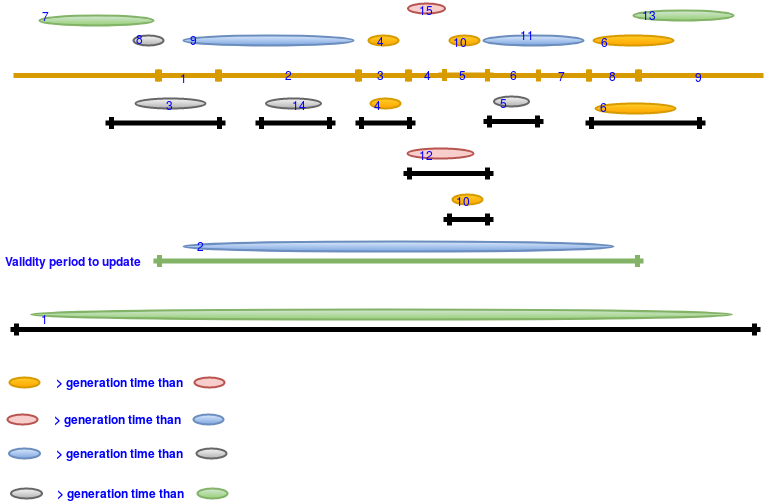
\includegraphics[width=150mm]{../fig/erase_and_replace_algorithm.png}
	\caption{Example of the effect of the erase and replace operation}
	\label{fg:erase_and_replace_algorithm}
  \end{center}
\end{figure}

\begin{table}[H]
\begin{tabular}{|M{0.07\linewidth}|M{0.15\linewidth}|M{0.15\linewidth}|M{0.15\linewidth}|M{0.15\linewidth}|M{0.15\linewidth}|M{0.15\linewidth}|}
\hline
Period & List to be created  & List to be created not ending on the current period & List to be removed & List of split & Marked as visible \\ \hline
1      & 7, 8                & -                                                   & 3                  & 1             & 2                 \\ \hline
2      & 7, 8                & -                                                   & 3, 14              & 1             & 2                 \\ \hline
3      & 7, 8, 9             & -                                                   & 3, 14              & 1, 2          & 4                 \\ \hline
4      & 7, 8, 9             & -                                                   & 3, 14              & 1, 2          & 4, 12             \\ \hline
5      & 7, 8, 9, 15         & -                                                   & 3, 12, 14          & 1, 2          & 4, 10             \\ \hline
6      & 7, 8, 9, 15         & 11                                                  & 3, 5, 12, 14       & 1             & 2, 4, 10          \\ \hline
7      & 7, 8, 9, 15         & 11                                                  & 3, 5, 12, 14       & 1             & 2, 4, 10          \\ \hline
8      & 7, 8, 9, 11, 15     & -                                                   & 2, 3, 5, 12, 14    & 1             & 4, 6, 10          \\ \hline
9      & 7, 8, 9, 11, 13, 15 & -                                                   & 2, 3, 5, 12, 14    & 1             & 4, 6, 10          \\ \hline
\end{tabular}
\caption{Table showing the steps done by the erase and replace algorithm}
\label{tb:erase_and_replace_algorithm}
\end{table}


\subsection {EVENT\_KEYS method}

The algorithm used to insert events using the method EVENT\_KEYS is a lot less complex than the algorithm used to insert events using the method ERASE\_and\_REPLACE.
The events and the associated keys are firstly inserted flagged as not visible. The method after applying the algorithm described bellow is in charge of deleting the events or making them visible, as well as making the event keys visible.
This method considers the generation time of the source associated to the events just inserted and its DIM signature assciated joint with every event key.
The steps are as follows:

\begin{enumerate}

\item The algorithm iterates over the pairs (event key, DIM signature UUID)
\item \label{for_each_pair} For each pair associated to events inserted with mode EVENT\_KEYS, the algorithm gets the first event associated to the event key and the DIM signature UUID which source has the maximum generation time
\item The algorithm deletes the rest of events associated to the event key and the DIM signature UUID and which source is different than the source of the previous event
\item The algorithm makes visible the events and the event keys associated
\item The algorithm goes to step \ref{for_each_pair}
\end{enumerate}

\section{Annotations ingestion}

Annotations are inserted associated to their explicit references and their annotation configuration.
The method followed for inserting annotations is similar to the method used for inserting events using the method EVENT\_KEYS.
The annotations are firstly inserted flagged as not visible. The method after applying the algorithm described bellow is in charge of deleting the annotations or making them visible.
The steps are as follows:

\begin{enumerate}

\item The algorithm iterates over the tubles (annotation configuration name, annotation configuration system, explicit reference)
\item \label{for_each_tuple} For each tuple associated to an inserted annotation inserted, the algorithm gets the first annotation associated to the annotation configuration and the explicit reference which source has the maximum generation time
\item The algorithm deletes the rest of annotations associated to the annotation configuration and the explicit reference and which source is different than the source of the previous annotation
\item The algorithm makes visible the annotations
\item The algorithm goes to step \ref{for_each_tuple}
\end{enumerate}




% Testing environment
\chapter{GSDM testing environment}\label{c:install_gsdm}

Inside the repository of the \acrshort{gsdm} component there is a \href{https://www.vagrantup.com/}{Vagrant} configuration file so that the environment for testing can be created automatically.

For doing so, follow the next steps:

\begin{enumerate}

\item Clone the repository

\begin{lstlisting}[breaklines=true, style=bash]

$ git clone https://bitbucket.org/dbrosnan/gsdm.git

\end{lstlisting}

\item Enter into the repository folder

\begin{lstlisting}[breaklines=true, style=bash]

$ cd (PATH_TO_GSDM)/gsdm

\end{lstlisting}

\item Run vagrant (see installation instructions in the referenced link)

\begin{lstlisting}[breaklines=true, style=bash]

$ vagrant up centos

\end{lstlisting}

\end{enumerate}

This will create a virtual machine with all you need to test the GSDM component.

In order to check that the component has been correctly installed, run the following commands to execute the automated tests:

\begin{lstlisting}[breaklines=true, style=bash]]

$ vagrant ssh centos
$ cd /vagrant/src/
$ py.test -v --cov-report html:tests/tmp/code_coverage_analysis --cov=gsdm tests

\end{lstlisting}

In order to check the coverage report, check Annex 1 and install firefox and open the code coverage analysis report:

\begin{lstlisting}[breaklines=true, style=bash]]

$ sudo yum install firefox
$ firefox tests/tmp/code_coverage_analysis/index.html

\end{lstlisting}

\section {Connecting to vagrant with X11 forwarding}

Read these links for detailed information:

\begin{itemize}

\item \href{https://coderwall.com/p/ozhfva/run-graphical-programs-within-vagrantboxes}{Run graphical programs within Vagrantboxes} 
\item \href{https://www.cyberciti.biz/faq/how-to-fix-x11-forwarding-request-failed-on-channel-0/}{Install X authority file utility} 

\end{itemize}

Allow X-Forwarding in your Vagrantfile:

To use X-Forwarding, you first need to allow it from within your Vagrantfile, like this:

\begin{lstlisting}[breaklines=true, style=bash]]

Vagrant.configure(2) do |config|
  ...
  config.ssh.forward_x11 = true
end

\end{lstlisting}

To be able to execute GUIs in the ssh session, you have to install xauth inside the virtual machine created:

\begin{lstlisting}[breaklines=true, style=bash]]

sudo yum install xauth

\end{lstlisting}

Now on your host run this:

\begin{lstlisting}[breaklines=true, style=bash]]

$ vagrant ssh-config
Host some_site
  HostName 127.0.0.1
  User vagrant
  Port 2222
  UserKnownHostsFile /dev/null
  StrictHostKeyChecking no
  PasswordAuthentication no
  IdentityFile vagrant.d/insecure_private_key
  IdentitiesOnly yes
  LogLevel FATAL
  ForwardX11 yes

\end{lstlisting}

Now you can ssh with X11 forwarding:

\begin{lstlisting}[breaklines=true, style=bash]]

ssh -X -p 2222 vagrant@localhost -i vagrant.d/insecure_private_key

\end{lstlisting}



% Create ingestion processor
\chapter{Create ingestion processor}

In the following chapter, the process of creating a processor for ingesting data to the \acrshort{eboa} module is explained.

The explanation is based on an example for ingesting Sentinel-2 data from the planning system (data received on NPPF files, xml formatted).

The example will use the python interface of the component, as the target version of the \acrshort{eboa} used in this explanation is the 0.1.0 and it is the only interface available.

\section{Installing EBOA on vagrant}

See the details in section \ref{c:install_eboa}.

\section{Structure of the folders and location of ingestion processors inside the project}

The ingestion processors are being located for the moment in the folder:

\begin{lstlisting}[breaklines=true, style=bash]]

src/ingestions

\end{lstlisting}

Inside this folder there is the folder s2 where the example explained here can be located:

\begin{lstlisting}[breaklines=true, style=bash]]

src/ingestions/s2/ingestion_nppf

\end{lstlisting}

There, the code of the processor, a folder for automated tests and a folder for input examples can be found:

\begin{lstlisting}[breaklines=true, style=bash]]

ingestion_nppf.py
input_files
tests

\end{lstlisting}

It is recommended to read the code inside the file ingestion\_nppf.py.

\section{Processor code}

For creating ingestion processors the \acrshort{eboa} component offers some helpers through the submodule ingestion which can be seen in the section \ref{\detokenize{eboa.ingestion:module-eboa.ingestion.functions}}.

The processor code has a main method:

\begin{lstlisting}[breaklines=true, style=python]]
def process_file(file_path):
    """Function to process the file and insert its relevant information
    into the DDBB of the eboa

    :param file_path: path to the file to be processed
    :type file_path: str
    """
\end{lstlisting}

Which should be provided as interface of the processor as in future versions it will be the main entry point to the processor.

This method shall extract from the file passed by parameter all the interesting information to the system.

The data extracted has to be formatted with the structure of a python dictionary which can be validated against a schema implemented in the engine side of the \acrshort{eboa} (method eboa.engine.engine.validate\_data). This data will be validated before treatement by the engine.

An example of the data structure, that has to follow the data to be inserted into the \acrshort{eboa}, can be seen in appendix \ref{ap:example_data_structure}.

For the version of this example of an ingestion processor, this method is called from the same phyton file from another method that is called from the main entry point to the file:

\begin{lstlisting}[breaklines=true, style=python]]
def command_process_file(file_path):
    # Process file
    data = process_file(file_path)
    ...

if __name__ == "__main__":
    ...

    returned_value = command_process_file(file_path)
\end{lstlisting}

Once the data has been extracted the method command\_process\_file(file\_path) will interface with the Engine of the \acrshort{eboa} to insert the data:

\begin{lstlisting}[breaklines=true, style=python]]
    # Process file
    data = process_file(file_path)

    engine = Engine()
    # Validate data
    filename = os.path.basename(file_path)

    # Treat data
    returned_value = insert_data_into_DDBB(data, filename, engine)
\end{lstlisting}

\section{Extraction of data}

\subsection{Extraction from an XML file}

The example provided performs the extraction of data from an XML file. To do so, the module uses the library \href{https://pypi.org/project/lxml/}{lxml}.

The following list includes a brief description of main operations available using this library:

\begin{itemize}
\item Importing the module:
\begin{lstlisting}[breaklines=true, style=python]]
# Import xml parser
from lxml import etree
\end{lstlisting}
\item Obtain Xpath object for reading the XML using XML paths:
\begin{lstlisting}[breaklines=true, style=python]]
    file_name = os.path.basename(file_path)
    parsed_xml = etree.parse(file_path)
    xpath_xml = etree.XPathEvaluator(parsed_xml)
\end{lstlisting}
\item Get nodes of an XML:
\begin{lstlisting}[breaklines=true, style=python]]
    record_operations = xpath_xml("/Earth_Explorer_File/Data_Block/List_of_EVRQs/EVRQ[RQ/RQ_Name='MPMMRNOM' or RQ/RQ_Name='MPMMRNRT']")
\end{lstlisting}
\item Perform operations with one node:
\begin{lstlisting}[breaklines=true, style=python]]
    generation_time = xpath_xml("/Earth_Explorer_File/Earth_Explorer_Header/Fixed_Header/Source/Creation_Date")[0].text.split("=")[1]
\end{lstlisting}
\end{itemize}

\section{Manual execution of the processor}

The processor can be manually executed passing the file path to be processed as follows:

\begin{lstlisting}[breaklines=true, style=bash]]

$ cd /vagrant/src/ingestions/s2/ingestion_nppf
$ python3 ingestion_nppf.py -f input_files/S2B_OPER_MPL__NPPF__20180727T110000_20180813T140000_0001.EOF

\end{lstlisting}

\section{Automated tests}

Inside the folder tests, there should be a python file which would cover the unit testing of the processor. For the example explained in this page, to execute the tests, run the following command:

\begin{lstlisting}[breaklines=true, style=bash]]

$ cd /vagrant/src/ingestions/s2/ingestion_nppf
$ py.test -v --cov-report html:tests/tmp/code_coverage_analysis --cov=ingestions tests/

\end{lstlisting}

Then, the code coverage analysis may be checked (following the instructions shown in the section \ref{x11_forwarding} and installing firefox) with the following command:

\begin{lstlisting}[breaklines=true, style=bash]]

$ firefox tests/tmp/code_coverage_analysis/index.html

\end{lstlisting}

\subsection{Creating the tests}

For validating the correct behaviour of the ingestion processor, automated tests should be provided which would cover completely the code of the ingestion processor.

For doing this, the provided solution makes use of the library unittest. With this library the utility py.test can detect all the tests inside a project, execute them and provide analysis on the failures.

The following list includes a brief description of main operations available using this library:

\begin{itemize}
\item Import the module:
\begin{lstlisting}[breaklines=true, style=python]]
import unittest
\end{lstlisting}
\item Define class for testing:
\begin{lstlisting}[breaklines=true, style=python]]
class TestEngine(unittest.TestCase):
\end{lstlisting}
\item Define the main method which will be executed every time before a unit test is executed:
\begin{lstlisting}[breaklines=true, style=python]]
    def setUp(self):
        # Create the engine to manage the data
        self.engine_eboa = Engine()
        self.query_eboa = Query()

        # Create session to connectx to the database
        self.session = Session()

        # Clear all tables before executing the test
        for table in reversed(Base.metadata.sorted_tables):
            engine.execute(table.delete())
\end{lstlisting}
\item Define unit tests:
\begin{lstlisting}[breaklines=true, style=python]]
    def test_insert_insert_nppf(self):
        filename = "NPPF_CONTAINING_ALL_DATA_TO_BE_PROCESS.EOF"
        file_path = os.path.dirname(os.path.abspath(__file__)) + "/inputs/" + filename

        ingestion.command_process_file(file_path)

        # Check that events before the queue deletion are not inserted
        events_before_validity_period = self.session.query(Event).filter(Event.stop < "2018-07-20T13:40:00.000").all()

        assert len(events_before_validity_period) == 0
\end{lstlisting}
\end{itemize}


\begin{appendices}

% XML schema
\chapter{XML schema}\label{ap:xml_schema}

The \acrshort{gsdm} offers schema validation for the inputs. In this section the XML schema (XSD) is shown:

\lstinputlisting[style=xml]{../../src/schemas/gsd_schema.xsd}


% JSON and Python schema
\chapter{JSON and Python data schemas}\label{ap:json_schema}

The \acrshort{eboa} offers schema validation for the inputs. 

The JSON schema is shown here:

\lstinputlisting[style=python]{../../src/schemas/eboa_schema.json}

Due to bad performances using the JSON schema, the \acrshort{eboa} implements a parsing method using Python, that is quicker. The performance is better even than the XSD for XML input data. For more details check the file \href{https://bitbucket.org/dbrosnan/eboa/src/master/src/eboa/engine/parsing.py}{src/eboa/engine/parsing.py}.


% Why using UUIDs
\chapter{Why UUIDs as primary keys instead of auto-increment IDs?}

Designs of relational databases must have a secure out of conflicts way of identifying entities inside the database. One possible solution for this is using auto-increment functions of the database to provide this secure out of conflicts way of identifying entities.

Using the auto-increment functions, though, implies a huge problem: the information has to be inserted in a sequential way so that the foreign keys are built by the database manager (PostgreSQL in this case).

A solution implemented in the data model of the \acrshort{gsdm} is using \acrshort{uuid}s (version 1).

The version 1 of the UUID (according to RFC 4122) is composed by the following fields: 

\begin{lstlisting}[style=bash, caption={XML input example for showing the values structure management.}]

        time_low                the first 32 bits of the UUID
        time_mid                the next 16 bits of the UUID
        time_hi_version         the next 16 bits of the UUID
        clock_seq_hi_variant    the next 8 bits of the UUID
        clock_seq_low           the next 8 bits of the UUID
        node                    the last 48 bits of the UUID

        time                    the 60-bit timestamp
        clock_seq               the 14-bit sequence number
        
\end{lstlisting}

Where the implementation of Python of this version according to the RFC is thread safe due to the following code:

\begin{lstlisting}[style=python, caption={Python code showing how the algorithm provides a mechanism for using UUIDs in a thread safe manner.}]

    global _last_timestamp
    import time
    nanoseconds = int(time.time() * 1e9)
    # 0x01b21dd213814000 is the number of 100-ns intervals between the
    # UUID epoch 1582-10-15 00:00:00 and the Unix epoch 1970-01-01 00:00:00.
    timestamp = int(nanoseconds/100) + 0x01b21dd213814000
    if _last_timestamp is not None and timestamp <= _last_timestamp:
        timestamp = _last_timestamp + 1
    _last_timestamp = timestamp
    
\end{lstlisting}

As \_last\_timestamp is global, this is visible to all the threads of the same process so that they will never see the same timestamp value.

But, this is still not multiprocessing safe. For making the UUIDs creation multiprocessing safe, the UUID has been enforced with the \acrshort{pid} of the process as the "node" field and a random number as the "clock\_seq".

So, this characteristic joint with the addition of the PID warranties the uniqueness of the UUIDs generated inside the GSDM.


\end{appendices}

\backmatter 

\clearpage

\printglossary[type=\acronymtype]

% \printglossary

\clearpage

\end{document}
